\documentclass{article}
\usepackage[UTF8]{ctex}
\usepackage{algorithm}
\usepackage{algpseudocode}
\usepackage{amsmath}
\usepackage{amssymb}
\usepackage{fancyhdr}
\usepackage{geometry}
\usepackage{sectsty}
\usepackage{tikz}

\xeCJKsetup{CJKmath=true}

\geometry{left=2cm, right=2cm, top=2cm, bottom=2cm}
\sectionfont{\fontsize{12pt}{15pt}\selectfont}

\title{机器学习——第三次作业}
\author{Koorye}
\date{2024年3月16日}

\pagestyle{fancy}
\fancyhead[L]{机器学习——第三次作业}
\fancyhead[R]{Koorye}
\fancyfoot[R]{基于\LaTeX 排版制作}

\begin{document}
\maketitle
\thispagestyle{fancy}

\section{试写出偏置-方差分解中这两部分的公式并说明它们的含义,说明模型复杂度与偏置、方差以及过拟合、欠拟合间的关系。}

\begin{equation}
    \mathbb{E}_\mathcal{D}[\{y(x;\mathcal{D})-h(x)\}^2]=\underbrace{\{\mathbb{E}_\mathcal{D}[y(x;\mathcal{D})]-h(x)\}^2}_{bias^2}+\underbrace{\mathbb{E}_\mathcal{D}[\{y(x;\mathcal{D})-\mathbb{E}_\mathcal{D}[y(x;\mathcal{D})]\}^2]}_{variance}+\underbrace{\epsilon^2}_{noise},
\end{equation}

简单表示为

\begin{equation}
    \text{expected loss} = \text{bias}^2 + \text{variance} + \text{noise}.
\end{equation}

如上式所示,偏置-方差分解是指模型的期望预测误差可以分解为偏置、方差和噪声三部分。其中:

\begin{enumerate}
    \item \textbf{偏置}:所有数据集的平均预测与预期的回归函数之间的差异。度量了某种学习算法的平均估计结果所能逼近学习目标的程度,反映模型的准确程度。
    \item \textbf{方差}:模型给出的解在平均值附近的波动。度量了在面对同样规模的不同训练集时,学习算法的估计结果发生变动的程度,反映模型的敏感程度。
\end{enumerate}

模型复杂度与偏置、方差以及过拟合、欠拟合之间的关系是:

\begin{enumerate}
    \item 偏置越\textbf{低},模型复杂度越\textbf{高}。因为模型越复杂,越能逼近学习目标。
    \item 偏置越\textbf{高},模型复杂度越\textbf{低}。因为模型越简单,越难以学习目标。
    \item 方差越\textbf{低},模型复杂度越\textbf{低}。因为模型越简单,越不容易受到不同数据集的影响。
    \item 方差越\textbf{高},模型复杂度越\textbf{高}。因为模型越复杂,越容易受到不同数据集的影响。
\end{enumerate}

\section{介绍分类的三类方法及其特点,并列举每类的具体方法。}

三类方法有:
\begin{enumerate}
    \item \textbf{判别函数}:直接找到一个函数$f(x)$,把每个输入$x$直接映射为类别标签。方法有\textbf{Fisher判别函数、感知机、SVM}等。
    \item \textbf{概率判别式模型}:直接对后验概率$p(C_k|x)$建模,再使用决策论来确定每个输入$x$的类别标签。方法有\textbf{Logistic回归、神经网络}等。
    \item \textbf{概率生成式模型}:先对类条件密度$p(x|C_k)$和先验类概率分布$p(C_k)$建模,再使用贝叶斯定理计算厚颜类概率分布$p(C_k|x)$。
          $$
          p(C_k|x)=\frac{p(x|C_k)p(C_k)}{p(x)},
          $$
          最后使用决策论确定每个输入$x$的类别。方法有\textbf{朴素贝叶斯分类器}等。
\end{enumerate}

其中1和2的特点是计算量小,但是容易过拟合;3的特点则是计算量大,但是不容易过拟合。

\section{有以下8个关于客户的身高,体重,鞋码和性别的样本,现有一位身高“中”,体重“中”,鞋码“中”的客户,试用朴素贝叶斯方法估计该客户的性别。}

\begin{table}[h]
    \centering
    \begin{tabular}{|c|c|c|c|c|}
        \hline
        编号 & 身高 & 体重 & 鞋码 & 性别 \\
        \hline
        1 & 高 & 重 & 大 & 男 \\
        2 & 高 & 中 & 大 & 男 \\
        3 & 中 & 中 & 大 & 男 \\
        4 & 中 & 中 & 中 & 男 \\
        5 & 矮 & 轻 & 小 & 女 \\
        6 & 矮 & 轻 & 小 & 女 \\
        7 & 矮 & 中 & 中 & 女 \\
        8 & 中 & 中 & 中 & 女 \\
        \hline
    \end{tabular}
\end{table}

首先求出先验概率$p(C_k)$:

\begin{equation}
    p(性别=男)=4/8,p(性别=女)=4/8。
\end{equation}

然后求出类条件概率$p(x|C_k)$:

\begin{equation}
\begin{split}
    p(身高=中|性别=男)=2/4, p(体重=中|性别=男)=3/4, p(鞋码=中|性别=男)=1/4, \\
    p(身高=中|性别=女)=1/4, p(体重=中|性别=女)=2/4, p(鞋码=中|性别=女)=2/4.
\end{split}
\end{equation}

最后得到后验概率$p(C_k|x)$:

\begin{equation}
\begin{split}
    p(性别=男|身高=中,体重=中,鞋码=中)=\frac{p(身高=中,体重=中,鞋码=中)p(性别=男)}{p(身高=中,体重=中,鞋码=中)} \\
    \propto p(身高=中|性别=男)p(体重=中|性别=男)p(鞋码=中|性别=男)p(性别=男) \\
    =\frac24\cdot\frac34\cdot\frac14\cdot\frac48=\frac{3}{64},
\end{split}
\end{equation}

\begin{equation}
\begin{split}
    p(性别=女|身高=中,体重=中,鞋码=中)=\frac{p(身高=中,体重=中,鞋码=中)p(性别=女)}{p(身高=中,体重=中,鞋码=中)} \\
    \propto p(身高=中|性别=女)p(体重=中|性别=女)p(鞋码=中|性别=女)p(性别=女) \\
    =\frac14\cdot\frac24\cdot\frac24\cdot\frac48=\frac{3}{32}.
\end{split}
\end{equation}

$\frac{3}{32}>\frac{3}{64}$,所以该客户的性别是\textbf{女}的概率更大。

\section{考虑一个硬间隔(hard margin)支持向量机和下面来自两类的训练样本:}
$$
+1: (2,2)\ (4,4)\ (4,0)
$$
$$
-1: (0,0)\ (2,0)\ (0,2)
$$

\textbf{(a) 画出这6个点,通过观察画出最优分类面和权向量w,给出分类面的方程w1x1+w2x2+b=0。计算出它的间隔margin(从分类面到最近数据点的距离)。}

\textbf{(b) 标出所有的支持向量,并说明原因?}

画出这6个点如下图所示:

\begin{figure}[h]
\centering
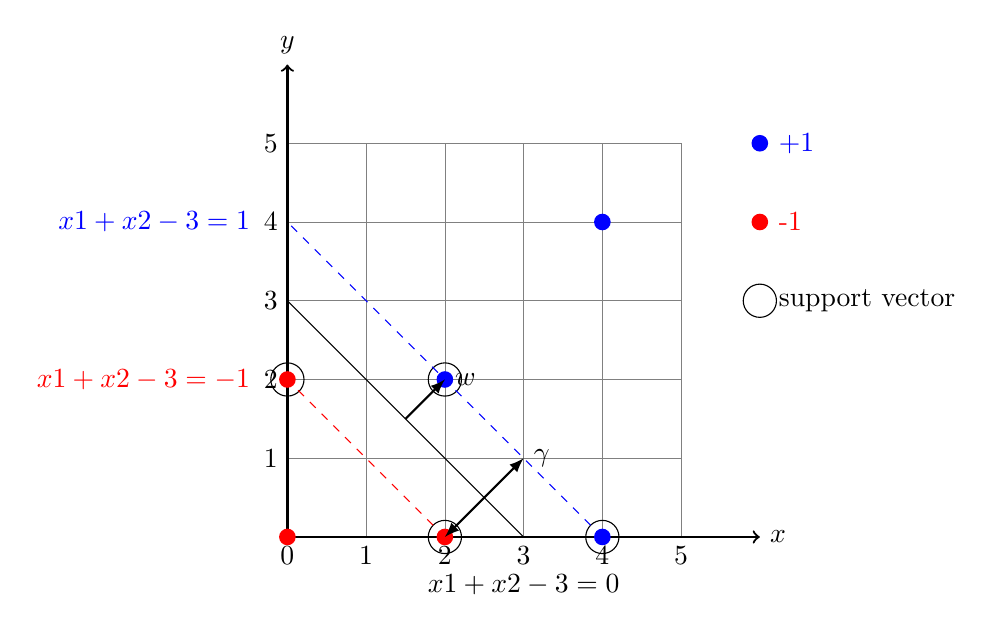
\begin{tikzpicture}
    \draw[help lines,step=1](0,0) grid (5,5);
    \draw[thick,->](0,0)--(6,0) node[right]{$x$};
    \draw[thick,->](0,0)--(0,6) node[above]{$y$};
    \foreach \x in {0,1,2,3,4,5}
        \draw (\x,0) node[below]{$\x$};
    \foreach \y in {1,2,3,4,5}
        \draw (0,\y) node[left]{$\y$};

    \fill[blue] (2,2) circle (3pt);
    \fill[blue] (4,4) circle (3pt);
    \fill[blue] (4,0) circle (3pt);

    \fill[red] (0,0) circle (3pt);
    \fill[red] (2,0) circle (3pt);
    \fill[red] (0,2) circle (3pt);

    \draw (2,2) circle (6pt);
    \draw (4,0) circle (6pt);
    \draw (0,2) circle (6pt);
    \draw (2,0) circle (6pt);

    \fill[blue] (6,5) circle (3pt) node[right]{\text{ +1}};
    \fill[red]  (6,4) circle (3pt) node[right]{\text{ -1}};
    \draw (6,3) circle (6pt) node[right]{\text{ support vector}};

    \draw (0,3)--(3,0) node[below=10]{$x1+x2-3=0$};
    \draw[dashed,color=red] (2,0)--(0,2) node[left=10]{$x1+x2-3=-1$};
    \draw[dashed,color=blue](4,0)--(0,4) node[left=10]{$x1+x2-3=1$};
    \draw[thick,latex-latex](2,0)--(3,1) node[right]{$\gamma$};

    \draw[thick,-latex](1.5,1.5)--(2,2) node[right]{$w$};
\end{tikzpicture}
\end{figure}

根据观察,最优分类面为$x1+x2-3=0$,间隔为$\gamma=\frac{2}{\Vert w\Vert}=\sqrt{2}$。从分类面到最近数据点的距离即为$\frac{\sqrt{2}}{2}$。

支持向量有$(2,2),(4,0),(0,2),(2,0)$,在图中被圈出。原因是这些点是离分类面最近的点,这些点决定了分类面的位置,而其他点对分类面的位置没有影响。

\end{document}